\documentclass{article}
\usepackage{amsmath}
\usepackage{amssymb}
\usepackage{graphicx}
\usepackage{hyperref}
\usepackage[version=4]{mhchem}

\title{Problem 4}
\date{}

\begin{document}
\maketitle

\section*{Problem}
\(A B\) is the diameter and \(E F\) is the chord of circle \(O . A C\) and \(B D\) are the distances from \(A, B\) to chord \(E F\), respectively. Show that \(C E\) \(=F D\).\\
\centering
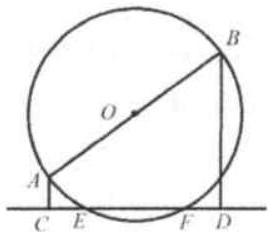
\includegraphics[width=\textwidth]{images/problem_image_1.jpg}

\section*{Solution}
Draw \(O M \perp E F\). \(M\) is the foot of the perpendicular from \(O\) to \(E F\).\\
Since \(A C \perp C D\). \(B D \perp C D, O M \perp E F, A C / / B D / / O M\).\\
Since \(A O=O B, C M=M D\)\\
Since \(O M\) bisects \(E F, E M=M F\)\\
(1) \(-(2): C E=F D\).\\
\centering
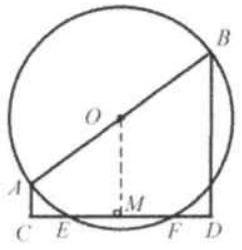
\includegraphics[width=\textwidth]{images/reasoning_image_1.jpg}

\end{document}
